\section{La mise en place d'un cache pour les zones peuplées}
\subsection{Introduction}

\subsection{Explications de la mise en place du cache}


\subsection{Résultats et observations sur le cache}


\subsection{Conclusion et perspectives du cache} 


La mise en place d'un cache pour les zones peuplées permettrait d'améliorer la réactivité dans un état (\textbf{W}) qui n'est pas encore améliorée. L'avantage de cette solution, même si l'issue n'est pas certaine, est de s'intéresser à une partie que l'on n'a pas encore fait évoluée. 
\par Le but de cette solution serait de mettre en place un cache qui garderait un certain nombre de nœuds qui vient de sortir de la liste des voisins du nœud. Ainsi comme les mouvements de l'avatar sont désordonnés, il est possible qu'il retourne vers des nœuds qu'il vient de quitter. Sur la figure~\ref{cacheW}, il est possible de se faire une idée de cette solution.

	\begin{figure}[!h]
        \centering
        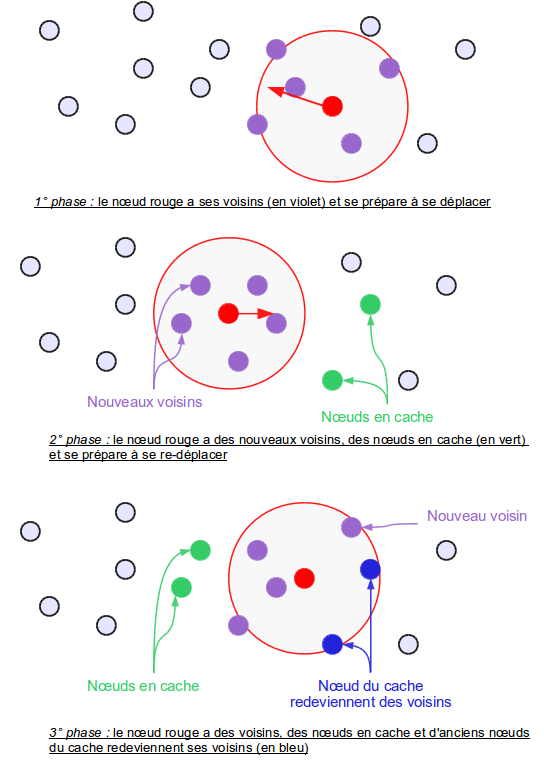
\includegraphics[scale=0.40]{./Ressources/Images/cacheW.png}
        \caption{Exemple de gain possible pour le prefetching}
        \label{cacheW}
        \end{figure} 

\par Sur la figure~\ref{cacheW}, un exemple de l'utilisation du cache est mis en avant. Nous pouvons voir trois phases durant lesquelles un nœud (rouge) va bouger et modifier ses voisins à chaque instant. Les nœuds, qui étaient voisins et qui ne le sont plus à l'instant suivant, sont placés dans le cache. Ainsi lorsque le nœud revient vers eux, ce dernier n'aura pas à refaire une recherche de voisins avec les deux nœuds verts, il aura juste à demander aux nœud verts si ils sont toujours au même endroit, etc.
\par Cette solution pourrait économiser des messages de découverte des voisins dans le cas de changements de direction fréquents. Mais l'efficacité de cette méthode n'est pas sûre. 

